\documentclass[11pt]{article}


\usepackage[utf8]{inputenc}
\usepackage[spanish]{babel}
\usepackage[T1]{fontenc}

\usepackage{tikz}
\usepackage{afterpage}
\usepackage{mathtools}
\usepackage{amssymb}
\usepackage{enumerate}
\usepackage{stackrel}
\usepackage{amsthm}
\usepackage{centernot}
\usepackage[a4paper, total={6in, 8in}]{geometry}
\usepackage{pgfplots}
\usepackage[toc,page]{appendix}
\usepackage{graphicx} % graficos

\newtheorem{teor}{Teorema} % Estilo de texto cursivo

\theoremstyle{definition} % Cambio del estilo de los teoremas a normal
\newtheorem{proposicion}{\textbf{Proposici\'on}}
\newtheorem{defi}{\textbf{Definición}}
\newtheorem{corolario}{Corolario}
\newtheorem{figura}{Figura}
\newtheorem*{lema}{Lema}
\newtheorem*{ejem}{\underline{Ejemplo}}
\newtheorem*{nota}{Nota}
\newtheorem*{observacion}{Observación}

\newcommand{\R}{\mathbb{R}}
\newcommand{\e}{\mathrm{e}}
\newcommand{\N}{\mathbb{N}}
\newcommand{\Q}{\mathbb{Q}}
\newcommand{\C}{\mathbb{C}}
\newcommand{\Cgot}{\mathcal{C}}
\newcommand{\dom}{\mathrm{Dom\ }}
\newcommand{\gradiente}{\bigtriangledown}
\newcommand{\nimplies}{\centernot\implies}
\newcommand{\nimpliedby}{\centernot\impliedby}
\newcommand{\nlongrightarrow}{\centernot\longrightarrow}
\newcommand{\nsubset}{\centernot\subset}
\newcommand{\oversim}[1]{\stackbin{_\sim}{#1}}
\newcommand{\sucesion}[2]{\left\{#1_{#2}\right\}^\infty_{#2 = 1}}
\newcommand{\sucesionelement}[2]{\left\{#1\right\}^\infty_{#2 = 1}}
\newcommand{\doubleright}[2]{ \left. \begin{array}{ll}	#1 \\	#2 \\	\end{array} 	\right\} }
\newcommand{\doubleleft}[2]{ \left\{\begin{array}{ll}	#1 \\	#2 \\	 \end{array}	\right. }
\newcommand{\doubleleftright}[2]{ \left\{\begin{array}{ll}	& #1 \\	& #2 \\	 \end{array}	\right\}}
\newcommand{\double}[2]{ \left. \begin{array}{ll}	#1 \\	#2 \\	 \end{array}	\right. }	
\newcommand{\tripleright}[3]{ \left. \begin{array}{ll}	#1 \\#2 \\#3\\	\end{array} 	\right\} }
\newcommand{\triple}[3]{ \left. \begin{array}{ll}	#1 \\#2 \\#3\\	\end{array} 	\right. }
\newcommand{\ximplies}[2]{\stackbin[#2]{#1}\implies}
\newcommand{\xiff}[2]{\stackbin[#2]{#1}\iff}
\newcommand{\ximpliedby}[2]{\stackbin[#2]{#1}\impliedby}
\newcommand{\dotproduct}[2]{<#1,#2>}
\newcommand{\norm}[1]{\left|\left|#1\right|\right|}
\newcommand{\function}[3]{#1\colon #2\to #3}
\newcommand{\xfunction}[4]{\stackbin[#4]{}{#1\colon #2\longrightarrow #3}}
\newcommand{\limite}[2]{\stackbin[#2]{\ }\lim\ #1}
\newcommand{\limited}{\stackbin{n\rightarrow\infty}\longrightarrow}
\newcommand{\xtiende}{x\rightarrow x_0}
\newcommand{\ntiende}{n\rightarrow\infty}
\newcommand{\ttiende}{t\rightarrow 0}
\newcommand{\htiende}{h\rightarrow 0}
\newcommand{\vacio}{\emptyset}
\newcommand\blankpage{%
    \null
    \thispagestyle{empty}%
    \addtocounter{page}{-1}%
    \newpage}




\title{Imágenes polinómicas de espacios reales}
\date{}
\author{Javier Pellejero Ortega}

\begin{document}

%----------------------------------
\maketitle
%-------------------------------------------------------

\section{Introducción}
Primero realizaremos un resumen de la charla introduciendo los conceptos e ideas desarrollados por José Fernando, Gamboa y Ueno.

\subsection{Imágenes polinómicas de espacios reales}

Queremos estudiar las imágenes de funciones $\xfunction{f}{\R^n}{\R^m}{x=(x_1,...,x_n)\to(f_1(x),...,f_m(x))}$ donde $f_i$ es una función polinómica.\\

Un ejemplo sencillo de este tipo de funciones, vistas en esta asignatura, son las aplicaciones afines:
\[(x_1,...,x_n)\mapsto(a_{01}+a_{11}x_1+...+a_{n1}x_n,...,a_{0m}+a_{1m}x_1+...+a_{nm}x_n)\]

Para dicho estudio tenemos una ayuda; el \textbf{Teorema \textit{Tarski-Seidenberg}} que nos dice, que en las condiciones anteriores, la imagen $f(\R^n)$ es un \textbf{conjunto semialgebraico} $\mathcal{S}\subset\R^m$. Un conjunto semialgebraico de $\R^m$ no es más que un conjunto que se puede definir con ecuaciones polinómicas del tipo $P(x)=0$ e inecuaciones polinómicas del tipo $Q(x) > 0$.\\

Estamos preparados para introducir el primer problema a tratar, el del \textbf{cuadrante abierto}: $Q=\{x>0, y>0\}$. Queremos determinar si existe $\function{f}{\R^2}{\R^2}$ polinómica tal que $f(\R^2)=Q$.

\begin{ejem} La relativa facilidad de la solución del \textbf{cuadrante cerrado} $\{x\geq 0, y\geq 0\}$ dada por $\xfunction{f}{\R^2}{\R^2}{(x,y)\to(x^2,y^2)}$ puede hacernos pensar que la del cuadrante abierto seguirá una estrategia similar; Sin embargo, nos equivocaríamos.
\end{ejem}

Una posible estrategia a seguir para cubrir $Q$ podría ser buscar una $\function{f_1}{\R^2}{\R}$ estrictamente positiva relativamente sencilla como $(x,y)\to((xy-1)^2+y^2)$ y buscar una $\function{f_2}{\R^2}{\R}$ de modo que la imagen de $f=(f_1,f_2)$ tenga por imagen $Q$.\\

José Fernando prueba que tal $f_2$ no existe y poco después encuentra una solución muy compleja, donde los polinomios tienen grado 64. Más adelante, Ueno logra encontrar una solución ``más sencilla'' $(x,y)\to(x^2y^2+(x^2y+xy^2-1)^2(x^2+1),x^2y^2+(x^2y+xy^2-1)^2(y^2+1))$. Además, logra en su tesis notorios avances, pero en general son propiedades con malas caracterizaciones y de alta complejidad.\\

Para finalizar este apartado, comentamos una última propiedad que determina que los \textbf{exteriores} de polígonos conexos que no desconectan $\R^2$ son imagen polinómica de una función $\R^2\to\R^2$.

\subsection{Imágenes polinómicas de un balón de fútbol}

\textbf{Sturmfels} les propone estudiar si dado un polígono convexo compacto $\mathcal{P}\subset\R^2$ existe una función polinómica $\function{f}{\R^3}{\R^2}$ tal que $f(\overline{B_3}(0,1))=\mathcal{P}$. Es decir, queremos una encontrar una función polinómica f que satisfaga este tipo de tranformaciones.
\begin{center}
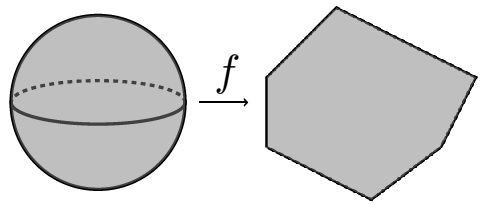
\includegraphics[scale=0.4]{1}\\\textbf{Figura 1}
\end{center}
Y para ello realizaremos una serie de transformaciones de funciones polinómicas, que sigan el siguiente diagrama:
\begin{center}
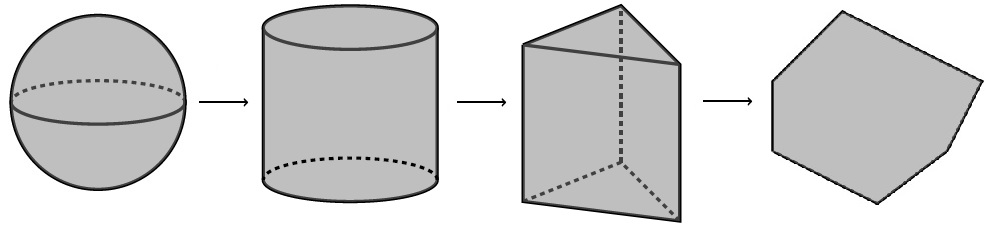
\includegraphics[scale=0.4]{2}\\\textbf{Figura 2}
\end{center}

La transformación que convierte el cilindro ($\{(x,y,z): x^2+y^2=1, -1\leq z\leq1\}$) en el prisma de base triangular ($\{(x,y,z): x\geq0,y\geq0, x+y\leq1, -1\leq z\leq1\}$) es la más sencilla, basta con aplicar $(x,y,z)\to(x^2,y^2,z)$.\\

La transformación de la esfera $\{(x,y,z):x^2+y^2+z^2 = 1\}$ en el cilindro es más compleja y viene dada por una doble transformación
\[(x_1,x_2,x_3)\mapsto(x_1,x_2,g(x_3))=(x_1,x_2,y)\mapsto	\big(x_1h(\norm{(x_1,x_2)}),x_2h(\norm{(x_1,x_2)}), y\big)\]
donde $g(t)=t(3-4t^2)$ y $h(t)=\dfrac{3}{\sqrt{3}}-\dfrac{4}{3\sqrt{3}}t^2$.\\

El caso de interés es el que finalmente nos lleva al polígono convexo (y por tanto a $\R^2$). Por ser un polígono convexo, podemos dividirlo en triángulos y a su vez podemos dividir en el prisma triangular en tantas secciones como triángulos hayamos generado en el polígono. Véase la \textbf{Figura 3} para una idea más clara de lo que queremos expresar

\begin{center}
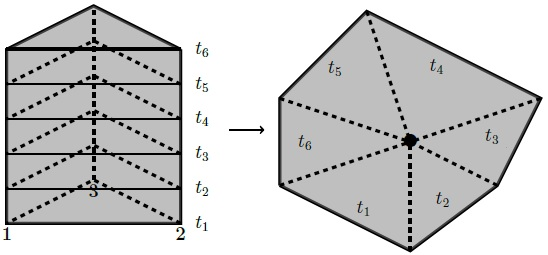
\includegraphics[scale=0.4]{3}\\\textbf{Figura 3}
\end{center}

Para no extendernos demasiado, no entraremos en detalle, pero la complejidad aquí reside en hacer corresponder cada uno de los $i$-triángulos del prisma con los del polígono mediante una función polinómica con el requisito de que los triángulos intermedios (con $t\in(t_i,t_{i+1})$) deben de tener sus vértices dentro del triángulo, una vez transformados. Esta última idea, puede verse reflejada gráficamente en la \textbf{Figura 4}, donde se ve como quedarían sobre el polígono (en forma de trayectoria) los triángulos con $t\in(t_1,t_2)$
\begin{center}
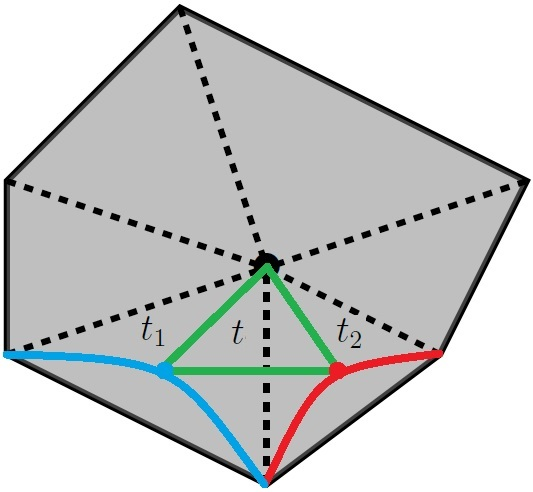
\includegraphics[scale=0.35]{4}\\\textbf{Figura 4}
\end{center}

\section{Valoración personal}
Entiendo que la caracterización de estos conjuntos semialgebraicos podría facilitar el estudio de ciertas funciones que parten de dichos conjuntos hacia un espacio euclídeo como $\R$.\\

No puedo evitar pensar en qué aplicaciones podría tener dichas caracterizaciones sobre problemas de programación lineal y en general de optimización. Las restricciones de dichos problemas representadas por ecuaciones e inecuaciones acaban por definir una región factible en el espacio que se corresponde con un polígono en un espacio $n$-dimensional y a los que se aplica una función objetivo $\function{f}{\R^n}{\R}$.\\

En el caso de la programación lineal, sabemos que el máximo (o mínimo) a buscar se encuentra en un vértice del polígono y pese a ello, los algoritmos tradicionalmente usados (como el \textit{Simplex}) tienen una complejidad muy alta en caso peor.\\

Sin embargo, en casos donde la no existe la linealidad de las restricciones, una caracterización de la región factible podría darnos una solución precisa del problema.



\end{document}